%!TEX root = ../main.tex

\chapter{Implementation}

\label{Chapter3-implementation}

This chapter is structured as follows: we begin by discussing some common high-level design decisions that apply to all of our implementations.
Secondly, we delve into the specifics of each key-value (KV) store, including their internals and implementation details.
Lastly, we demonstrate how we leveraged log-structuring to achieve the desired incremental snapshotting functionality of our key-value store.

\section{Common design decisions}

First of all, we go through some design decisions that are common throughout all of the implementations, namely the programming interface and encoding of values.

\subsection{Application Programming Interface}
\label{api}

We designed our implementations to expose a common interface (API) to the programmer.
By doing this we allow for easy benchmarking, testing, and ultimately a fair comparison between the engines.
The API is programmatically defined within a parent class that is inherited and extended by the classes corresponding to each engine, of which the exact method signatures can be found in appendix \ref{Appendix-A-code}.
The methods supported are:

\begin{itemize}
    \item \verb"get": For retrieving the value of a given key. This operation is called a \textit{read}.
    \item \verb"set": For setting the value of a given key. If the key does not exist, it is inserted in the database with the given value, and if it already exists it is updated to the given value. If the value is empty, this is considered a delete. We refer to all these operations as \textit{writes}.
    \item \verb"close": Closes the database by flushing all buffers and closing all files.
    \item \verb"snapshot": Takes a snapshot of the current state, by flushing all buffers and pushing the latest created files to a remote directory (more on that in section \ref{section-snapshots}). This method takes as argument an integer which is the snapshot identifier. The values of those integers should be unique and ascending but not necessarily consecutive, for example $1, 3, 6, 8$ is a valid sequence of snapshot identifiers for taking four consecutive snapshots, but $2, 5, 4, 8$ is not.

    \item \verb"restore": Using the remote directory, it pulls all files  associated with a given version, restoring the state of a specific point in time when a snapshot was taken. This method takes an integer as an optional argument, representing the snapshot version to restore. If the argument is not given, the latest version is restored by default.
\end{itemize}

The decision to treat deletes as mere writes to empty values offers significant advantages in terms of both usage and implementation. By adopting this approach, we eliminate the need to invoke special methods or follow complex deletion procedures. Instead, a straightforward write operation can be used to signify the deletion of a record. On the implementation side, treating deletes as writes to empty values allows us to avoid dealing with intricate concepts such as \textit{tombstones}. In certain database systems, tombstones are special markers used to indicate record deletions [\cite{myrocks}]. However, by adopting our chosen approach, we eliminate the need for tombstones altogether.

Also, all keys and values are in the form of raw bytes. This the design decision followed in the APIs of major commercial key-value stores too, like \cite{rocksdb} and \cite{redis}, because besides offering simplicity, it also allows for maximum flexibility, as any other data type can be serialized in bytes (and \textit{has} to be if it is to be written on disk), and makes the encoding of the key-value pairs on disk easy implementation-wise.

\subsection{Encoding}

Regarding the encoding of the key-value pairs on disk, we encode each key-value pair as shown in figure \ref{fig:encoding}: we first encode the length of the key in bytes, then we write the key itself, and then we repeat the same for the value. This enables us to avoid any kind of character-escaping mechanisms, special characters, or padding, which would all add complexity, restrictions, and would waste disk space.

\vspace{20px}
\begin{figure}[h]
    \centering
    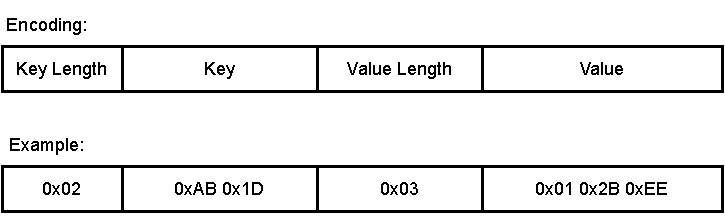
\includegraphics[width=0.9\textwidth]{encoding.pdf}
    \caption{Encoding \& Example. Keys and values are prepended by their respective length values.}
    \label{fig:encoding}
\end{figure}
\vspace{20px}

An important benefit from using such encoding is that it allows us to encode keys and values of arbitrary size without limit. The trade-off is that we use slightly extra disk space for the encoding bytes if the keys and/or values are large. With encoding bytes of length one we can have keys/values up to $2^{1*8}-1=255$ bytes long, with length two we can have up to $2^{2*8}-1=65535$ et cetera. Each key-value store accepts as argument in the constructor the maximum key length and the maximum value length, which we use to determine the amount of bytes we will use for the encoding.

\subsection{Filesystem and Persistence}

Another design decision is to store all data in files under one directory on disk, which enables easy backups and management in general.

Regarding the behavior of the key-value store upon initialization, if the key-value store is not initialized with a connection to a remote directory, and finds data in its local data directory from a previous run, it will rebuild its indices using this local data.

If on the other hand a key-value store is initiated with a remote connection (either a path in the same machine, which is expected to have been mounted remotely elsewhere, or \textit{minio} - more on that in section \ref{section-snapshots}), it will attempt to fetch the latest snapshot. If such a snapshot is available, it will overwrite any preexisting data in its local directory, giving preference to the snapshot.

\section{Log-Structured Merge-Tree}

The Log-Structured Merge-Tree (LSM-Tree) is a disk-based data structure [\cite{lsmtree}], and one of the most prominent, battle-tested, and well-researched database engines.
It was invented by Patrick O'Neil in 1996 and has since been used in multiple databases, such as Google's \cite{leveldb}, Meta's \cite{rocksdb} and Apache's \cite{cassandra}.
% TODO add the others from the paper I found recently.

The LSM-Tree makes extensive use of the \textit{log-structuring} technique, which first appeared in the LFS file system [\cite{lsm-filesystem}] and has since been used not only in LSM-Tree-based database management systems, but also in other types of storage engines, even B-Tree-based ones [\cite{llama}].

Log-structuring offers significant speedups by significantly reducing the number of writes per page and transforming them into a "sequential" format.
In other words, it consolidates numerous random writes into a single large multi-page write [\cite{llama}].

In this work, we use log-structuring extensively, because, besides its advantages in I/O operations, it also provides a straightforward way to create incremental snapshots of the database's state.
We analyze the way we leveraged log-structuring for incremental snapshotting later, in section \ref{section-snapshots}.

Given the close relationship between log-structuring and the LSM-Tree (which makes extensive use of it), we will introduce the concept in tandem with the LSM-Tree.

\subsection{Design}
\label{subsection-lsm-design}

The power of the LSM-Tree can be partially attributed to the fact that it uses lightweight indices, when compared to B-trees which effectively double the cost of every I/O operation to maintain their indices [\cite{lsmtree}].
This enables the LSM-Tree to scale to very high write and read rates.

However, one other important factor for the LSM-Tree's fast I/O is the use of an in-memory buffer, also called \textit{memtable}, which aggregates the updates and when it's full, it flushes them to disk sequentially.
As it is well known, disks perform much faster sequential operations that operations than require random-access, especially in the cloud, where inexpensive disks have limited I/O rates [\cite{llama}].

This buffer flushes the aggregated data into \textit{sorted} chunks of data that are commonly referred to as SSTs for ``Sorted String Tables'', but we will just call them ``runs''.
Sorting is essential for indexing, as it enables us to lookup keys in logarithmic time instead of linear.

\subsubsection{Writing data}

Initially, as we are writing data, we keep them in our buffer, and when this buffer is full, we flush it into a run-file. This can be seen in figure \ref{fig:lsm-flush}, where the file \verb"L0.0.run" is created, corresponding to the first file of the first run (everything is zero-indexed).

\vspace{20px}
\begin{figure}[h]
    \centering
    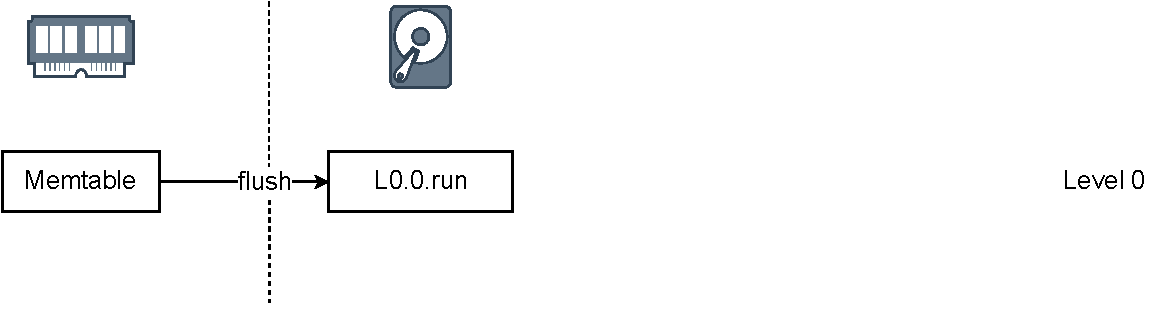
\includegraphics[width=1\textwidth]{lsm-flush.pdf}
    \caption{Example of LSM-Tree flushing.}
    \label{fig:lsm-flush}
\end{figure}
\vspace{20px}

As we continue writing key-value pairs, we create new runs in the same level by flushing our memtable (figure \ref{fig:lsm-flush2}), until their number reaches the maximum allowed runs per level, which is defined by the parameter \verb"max_runs_per_level" when instantiating the LSM-Tree. When that happens, a merge is triggered; the merge will merge these files into one file in the next level, and will check if the number of runs in that level is equal to the maximum runs per level. If it is, it will cascade the merging recursively to the next level, and this process will keep happening until no merges need to be done.

\vspace{20px}
\begin{figure}[h]
    \centering
    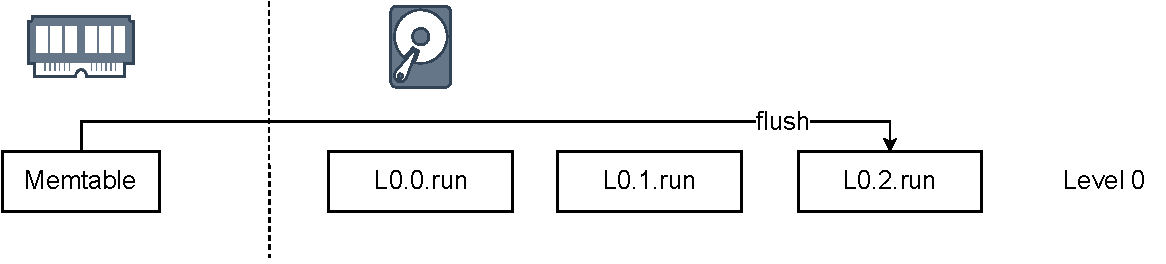
\includegraphics[width=1\textwidth]{lsm-flush2.pdf}
    \caption{Example of LSM-Tree flushing (cont.).}
    \label{fig:lsm-flush2}
\end{figure}
\vspace{20px}

The merging process is shown in figure \ref{fig:lsm-merge}, where the runs in the first level are merged into \verb"L1.0.run". After being merged, the files in the first level are deleted.
The merging process resembles the greedy merging step in the mergesort algorithm, because every run is sorted. We keep a number of file descriptors equal to the number of runs we are merging, and go through all of them at the same time. We take care to write the smallest key first, to make sure that the resulting merged file is also sorted. In case of two or more conflicting keys during the process, we write the latest one (the one with the largest run index) and skip the rest, as those have been overwritten by a more recent write and are not valid anymore. This is also how the LSM-Tree performs garbage-collection - during the merging process, invalid values are dropped.

\vspace{20px}
\begin{figure}[h]
    \centering
    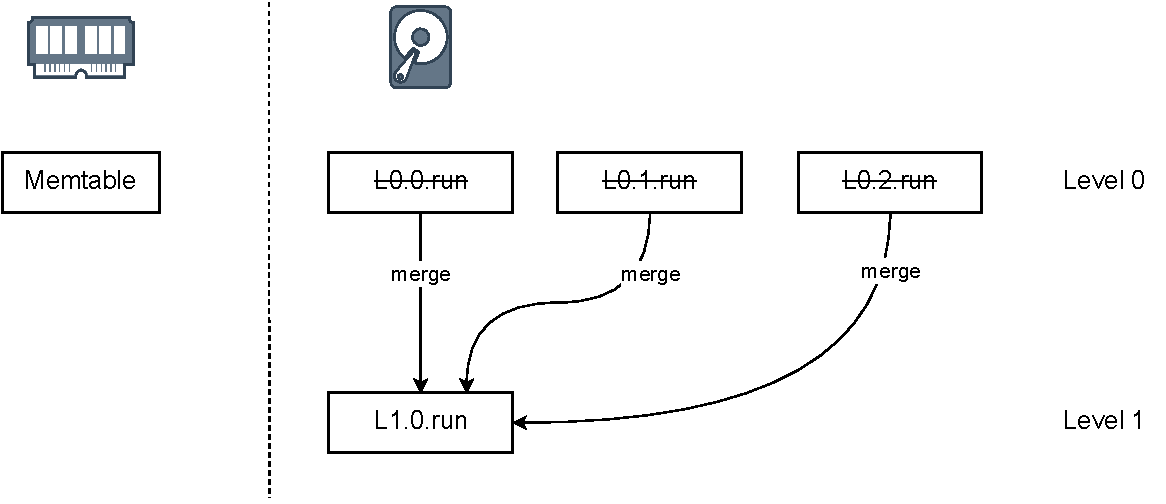
\includegraphics[width=1\textwidth]{lsm-merge.pdf}
    \caption{Example of LSM-Tree merging.}
    \label{fig:lsm-merge}
\end{figure}
\vspace{20px}

\subsubsection{Reading data}

To retrieve values using the \verb"get" operation, it is necessary to search through the files in reverse order to locate the latest write.
This involves performing a binary search on each file, starting from the first level, and then searching within each level from the runfile with the highest index to the lowest.

This search can be time-consuming if done on the files themselves, because it would involve a large number of I/O operations, so we use a data structure called \textit{fence pointers} [\cite{fence-pointers}] to speed up the process. The fence pointers are essentially sparse in-memory indices implemented with arrays that allow us to do binary-search in memory, and they associate a key with its offset in the runfile. Of course, they don't store all the keys, as that would be like keeping all the keys in memory and thus we would miss one of the main points of using an LSM-Tree. Instead, we use a subset of them, and since the runfile is itself sorted, if the key we are looking for does not have a fence pointer itself, we still know the offsets among which it should be (hence the name ``fence pointers'') and we can go ahead and search for it linearly on the file. The gap in numbers of key-value pairs between the offsets of the pointers is controlled via a parameter called \verb"density_factor" - the higher its value, the greater the gaps and the more key-value pairs we have to search sequentially on disk. An example illustrating how fence pointers function can be found in figure \ref{fig:fence-pointers}.

\vspace{20px}
\begin{figure}[h]
    \centering
    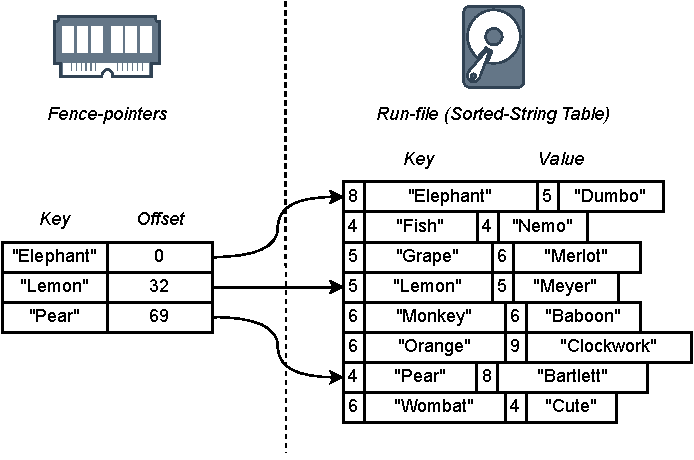
\includegraphics[width=1\textwidth]{fencepointers.pdf}
    \caption{Fence pointers example with density factor equal to 3, i.e. a pointer that maps a key to a file offset is created for every 3 entries of the SST.}
    \label{fig:fence-pointers}
\end{figure}
\vspace{20px}

The fence pointers offer a significant speedup, but we can skip entire runfiles if we know for sure that they don't contain the key we are looking for by using Bloom filters [\cite{bloom-filters}]. The Bloom filter is a probabilistic data structure that when queried if a key exists in a set (a runfile in our case) it will answer negatively with 100\% certainty if it does not. The positive answer is not always accurate, but having a few false positives is no problem for files that we were going to search anyway if we didn't have the Bloom filter.

The Bloom filter achieves this probabilistic lookup by employing a bitarray of $m$ bits and $k$ hash functions. To illustrate how it works, let us consider the example in figure \ref{fig:bloom-filter} with a bitarray of $m=20$ bits and $k=3$ hash functions.

\vspace{20px}
\begin{figure}[h]
    \centering
    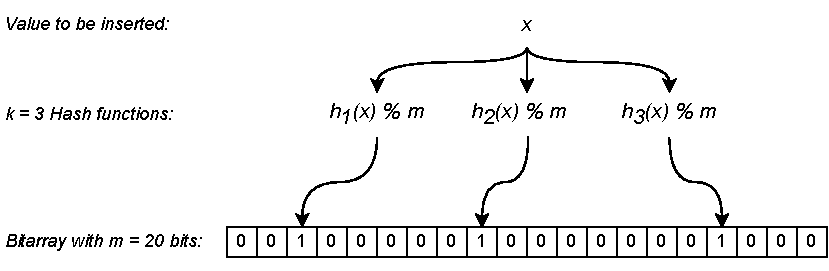
\includegraphics[width=1\textwidth]{bloomfilter.pdf}
    \caption{Bloom filter example with bitarray of 20 bits and 3 hash functions.}
    \label{fig:bloom-filter}
\end{figure}
\vspace{20px}

To insert value $x$, we hash it using all three hash functions obtaining the values $h_i(x), i=\{1,2,3\}$, then we calculate the values $p_i = h_i(x)\mod{m}$, and set the bits of the bitarray with positions equal to $p_i$ to $1$. When we want to query the Bloom filter, to check whether the value $x$ exists, we use the hash functions and modulo operation again the same way and check whether the bits at positions $p_i$ are set to 1. If there is at least one bit that is set to zero then $x$ definitely does not belong in the set of values inserted in the Bloom filter and if all values are set to one, then $x$ \textit{probably} belongs in the set. The positive answer is probabilistic simply because the same bits may have been set to 1 from insertions of values other than $x$.

The probability of getting a false positive answer from the Bloom filter is a function of the bitarray length $m$, the number of hash functions $k$, and the number of inserted elements $n$. Assuming that the hash functions are \textit{perfect} i.e. the probability distribution of the hash function values is uniform, we can calculate this probability. With some algebraic manipulation, we can also calculate \textit{the optimal number of hash functions $k$ and bitarray length $m$, given the number of elements to be inserted $n$ and the false-positive probability $\epsilon$}. These values are shown below, with $m$ being rounded up and $k$ rounded down for performance reasons, implementation-wise:

$$ m = \Bigl\lceil-\frac{n\ln \epsilon}{(\ln 2)^2}\Bigr\rceil $$
$$ k = \Bigl\lfloor \frac{m}{n}\ln 2 \Bigr\rfloor$$

The creation of Bloom filters and fence pointers occurs in-memory concurrently with the writing of a runfile, when flushing the memtable or when merging other runs. After the Bloom filters are created, they stay in-memory so that they can be queried for faster lookups, but we also persist them on disk by embedding them into the runfiles. If a system failure happens, the key-value store can quickly load all the fence pointers and Bloom filters from the disk without having to go through all the discovered files to rebuild them from scratch. This design decision significantly reduces the recovery time of the store at the expense of using (a bit) more disk space.

To embed the fence pointers and the Bloom filter into a runfile, we append each of them at its end along with two 64-bit values that correspond to their offsets in the runfile. These two offsets therefore define three segments in the run-file: the first is the SST, the second contains the fence pointers and the third is the Bloom filter.

After these additions, value retrieval looks as follows (see figure \ref{fig:lsm}): starting from the first level and from the rightmost latest run, we query the Bloom filters for the key we are looking for. When a Bloom filter answers positively, we query the fence pointers, and get an offset. We look up at most $d$ key-values in that file following this offset, where $d$ equals the density factor. If the key is not found, we repeat this process with the next runfile. If we exhaust the lookups and haven't found the key, we return the empty value (0 bytes).

\vspace{20px}
\begin{figure}[h]
    \centering
    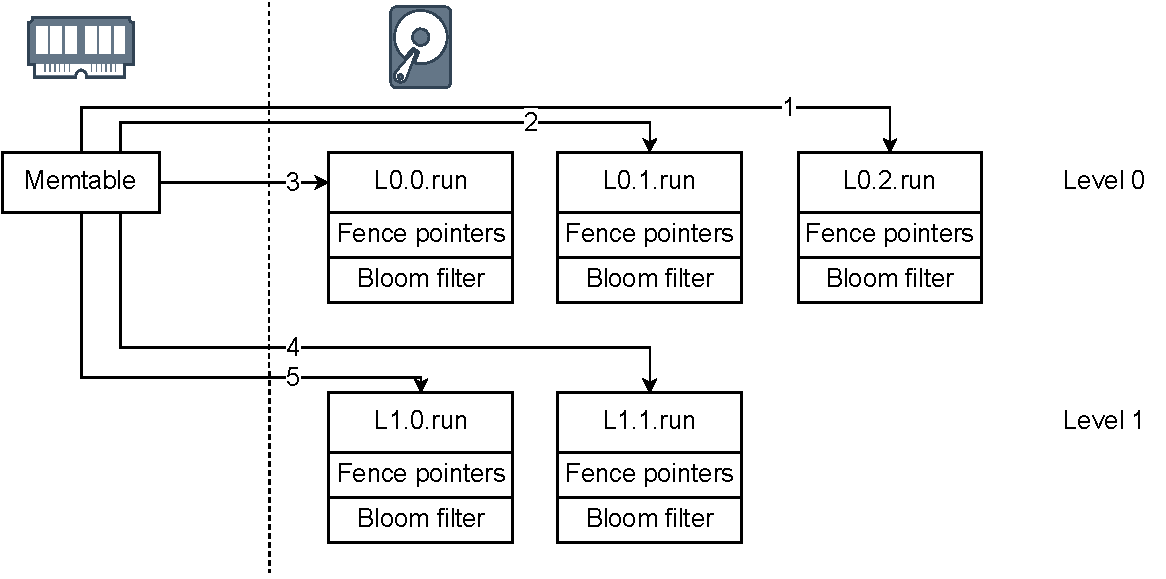
\includegraphics[width=1\textwidth]{lsm.pdf}
    \caption{Example of value retrieval in an LSM-Tree. The numbers in the arrows signify the search order.}
    \label{fig:lsm}
\end{figure}
\vspace{20px}

\subsubsection{Fault-tolerance}

As a final design choice, we add a write-ahead log (WAL) to make the database more resilient by preventing loss of unflushed records in the memtable in the event of a system failure.
More specifically, when we write a value to the store, we also write it to an append-only log. Since the log is append-only, it is still relatively fast despite the I/O, and at the same time it allows us to \textit{rebuild the memtable} by re-inserting the values after a system crash, making the database more fault-tolerant. 

\subsubsection{Tiering vs Leveling}

LSM-Trees come in two flavors, depending on the merging strategy: there are the LSM-Trees that use \textit{tiering} and those that use \textit{leveling} [\cite{compactionary}]. In tiering, we use up to $R$ runs per level, while in leveling we only use one.
As we increase $R$, the first level essentially transforms into an append-only log, which has the highest write speed. However, the reads become slower, as the LSM-Tree has to search a higher number of files to retrieve a value. On the other hand, in leveling when $R=1$, the LSM-Tree merges each file directly to the runfile of the next level, using the file sizes as thresholds that trigger merges. This optimizes the read performance but impedes the writes due to frequent merges [\cite{lsm-design-space}]. Figure \ref{fig:tiering-leveling} illustrates the difference between the tiering and leveling.

\vspace{20px}
\begin{figure}[h]
    \centering
    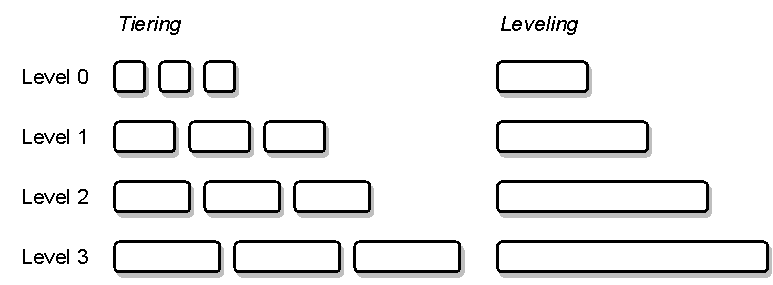
\includegraphics[width=1\textwidth]{tieringleveling.pdf}
    \caption{Tiering vs Leveling in LSM-Trees. Tiering sort-merges $R$ runs per level ($R=3$ in this example) into a run in the next level, while in leveling each run is greedily sort-merged with the run from the next level.}
    \label{fig:tiering-leveling}
\end{figure}
\vspace{20px}

Our implementation uses tiering because we are optimizing for writes. Nonetheless, the $R$ value described above is still configurable, and we will analyze the performance of the LSM-Tree for various values of it in Chapter \ref{Chapter4-evaluation}.

\subsection{Implementation}

As we stressed in the previous subsection, the properties of the LSM-Tree are derived primarily from having \textit{sorted} runfiles.
To remove the values from the memtable when flushing it in order, we need a data structure that does this operation efficiently.
% i can write this a bit better...
At the same time, we want this data structure to support efficient lookup and insertion/update of values.
These requirements are satisfied by Skip lists, or self-balancing binary-tree structures, like AVL trees and Red-Black trees. The skip list is used in some commercial LSM-Tree-based key-value stores, like \cite{leveldb} but operations on them are not guaranteed to be efficient due to their probabilistic nature. On the other hand, AVL trees and Red-Black trees have guaranteed access, lookup, insertion, and delete complexity of $\mathcal{O}(\log{}(n))$.

In our implementation, we used the \verb|sortedcontainers| package, a Python implementation of an associative array which offers the same complexity for the above operations. For the fence pointers, we used the same package because the fence pointers' keys have to be sorted \textit{to allow for efficient in-memory lookup}, with the binary-search algorithm.

For the Bloom filters, we could not use the most popular publicly available implementation due to a versioning incompatibility so we implemented it from scratch using a bitarray which is persisted using base64 encoding. As hash function we used MurmurHash3, a fast non-cryptographic hash function, which is a common choice for Bloom filters and other probabilistic data structures that require general hash-based lookups.

\section{AppendLog}

AppendLog is primarily based on \textit{Bitcask} [\cite{bitcask}], a log-structured hash-table key-value store. Bitcask constitutes one of the backend choices for Riak, a popular commerical distributed key-value store. It is an operationally and conceptually a simple database, but it is precisely its simplicity that makes it fast and robust.

\subsection{Design}

The AppendLog has two main components: a (log-structured) append-only log, and an in-memory hash-table.

To understand how it operates and its design, we will start with the writes.
Leaving aside log-structuring for now, we assume that we only use an append-only log, and we write key-value pairs to it.
For every key-value pair we write, we use the hash-table as an index which keeps track of the key-to-offset mapping in this log. The writes in this log are immutable - if we update a key to a new value, we just append it as a new key-value pair.

Then, to read the value of a key, we query the in-memory hash-table for key, get the offset, and seek to this offset and read the key-value pair.

This simple design is very fast because it writes data to the disk sequentially, and sequential I/O is faster in both mechanical and solid-state disks. In mechanical HDDs it is faster because the rotational parts of the disk do not have to seek to other positions so they do not add overhead, and in SSDs sequential writes mitigate the phenomenon of \textit{write-amplification} [\cite{write-amplification}] which we introduced in Chapter \ref{Chapter2-related-work}.

However, the design so far has a major drawback; it lacks garbage-collection.
As updates to values are appended, the old values are useless and only take up disk space.
To solve this issue, we introduce log-structuring to the design, which we have already used in the LSM-Tree implementation to solve a similar problem.
With log-structuring, we leverage the merging step to drop the old values.

Concretely, as we write values, we use a size-threshold value for the logfile size that when exceeded, we close the log file and start a new one. These logfiles are equivalent to the runfiles in the LSM-Tree's log-structuring scheme.
Then, we use a second parameter as the upper limit of the number of logfiles.
When this limit is reached, we merge the files in this run into a new file in the next level and at the same time we update the hash-table index to point to the new location.

This new design decision has the following implication: the index can no longer just point to an offset, as we have multiple files in our log-structured scheme.
The solution is to simply store the file information in the hash-table alongside the offset, so the index points to the offset of a specific file.

The entire design so far is visualized in figure \ref{fig:appendlog}.
In this figure, we see an example of a potential snapshot during the operation of an AppendLog instantiated with the parameter of maximum runs per level set to three and maximum key-value capacity per file set to two, right before the merging phase. The first level is full and thus the files \verb|L0.0.run|, \verb|L0.1.run| and \verb|L0.2.run| are about to be merged in \verb|L1.2.run|.
We notice how the index always points to the latest record.
In the next section (\ref{appendlog-implementation}) we explain how the merging is implemented.

Compared to the LSM-Tree, the AppendLog has the following advantages:
\begin{enumerate}
    \item It offers significantly faster reads, since a value retrieval is essentially a query to an in-memory hash-table, a seek to a file offset and a file read operation. There is no need to search multiple files or lookup multiple data structures.
    \item It is unencumbered by the overhead that the creation of the fence pointers and the Bloom filters add to the LSM-Tree.
    \item The hash-table index itself is faster than the LSM-Tree's insertions and deletions. The hash-table has an complexity for these operations of (amortized) $\mathcal{O}(1)$ while the memtable is $\mathcal{O}(\log{}(n))$, where $n$ is the number of entries to the memtable.
\end{enumerate}

The advantages however come at the following costs:
\begin{enumerate}
    \item The keys have to all fit in memory, since they have to be hosted to the hash-table. This hampers the scalability of the AppendLog.
    \item The AppendLog does not perform any buffering before flushing the entries to disk. In some cases this fact may degrade performance. We will analyze this further in the following section, \ref{appendlog-implementation}.
\end{enumerate}

To recover from a failure, the AppendLog needs to rebuild its main index. To do this, it has to scan all the files in reverse order (i.e. reverse to the order they are written) and for each key-value pair it needs to update the index. After this procedure, the index will point to the latest records.

\vspace{20px}
\begin{figure}[h]
    \centering
    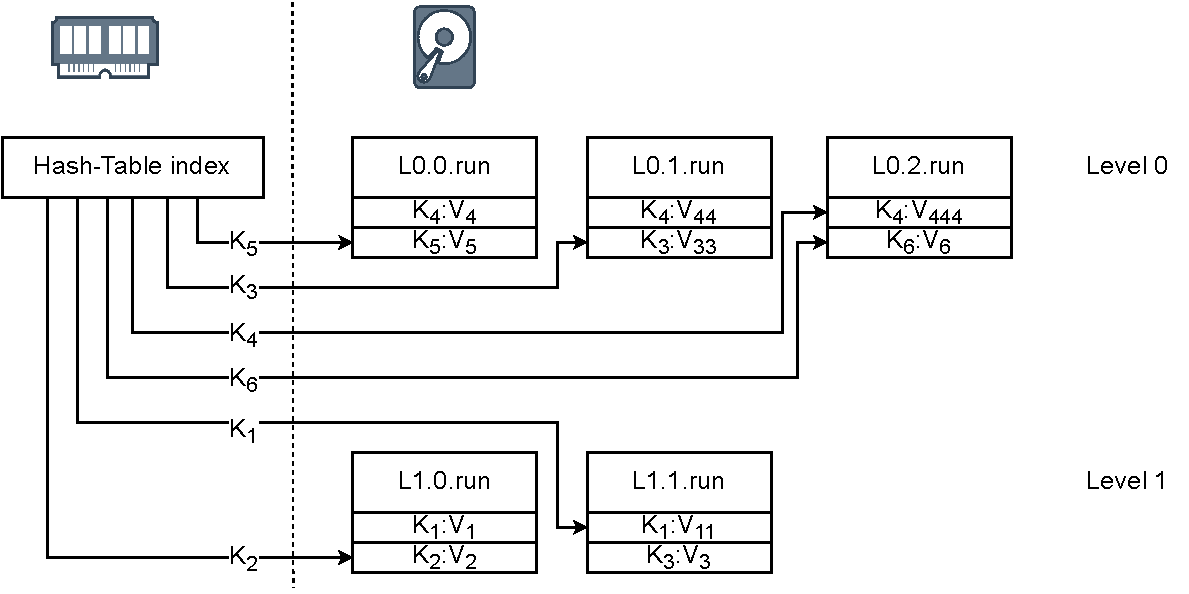
\includegraphics[width=1\textwidth]{appendlog.pdf}
    \caption{Example of operation of the AppendLog. $K_i$:$V_j$ are key-value pairs.}
    \label{fig:appendlog}
\end{figure}
\vspace{20px}

\subsection{Implementation}
\label{appendlog-implementation}

Although the implementation of the AppendLog is straightforward, it does feature certain intricacies that require attention, like the merging strategy and the record flushing.

Regarding merging, the resulting files need to be devoid of invalid records, i.e. key-value pairs that have been updated more recently. This step is important as it is the only garbage-collection mechanism. This can be done in multiple ways using extra memory, but there is in fact a way to achieve it using the already present index without extra memory or modifications. Concretely, for a single file, we read through the file sequentially, going over all the key-value pairs. For each key-value pair that we encounter, we query the index - if the offset that the index returns is equal to the current read offset of the file we are scanning, then this means that this record is indeed the latest for the queried key and must be preserved. Thus, we write it to the merged file, otherwise we drop it and continue to the next read. This process is repeated for the rest of the files in a level, resulting in a single merged file. After that, we can delete the merged files.

To improve the efficiency of the merging process in the AppendLog, we have implemented a garbage-collection mechanism called \textit{compaction} that is triggered right after flushing. This feature is optional and can be enabled as needed. By performing some of the garbage-collection work on flushed files before merging, we can distribute the total workload more evenly during the operation of the AppendLog. This, in turn, allows for faster and more streamlined merging, as some of the work that would typically be done during merging has already been completed. We evaluate the effectiveness of this mechanism in Chapter \ref{Chapter4-evaluation}.

One ramification of this merging algorithm is that it compels us to write the keys along with the values on disk, because we need to know the key associated with a value so that we can query the index appropriately, leading us to using more disk space. However, there is no other way to know which record is the latest (and at the same time make this information persistent) without using extra memory, which is more expensive than the disk and also volatile. This is also the approach that Bitcask follows [\cite{bitcask}].

When implementing the AppendLog, we used a profiler to look for bottlenecks. Evidently, the \textit{open()} system call adds significant overhead to I/O operations. This led us to keep the files open for reading (and for writing where applicable) and keep their file descriptors available in memory at all times. The files are then closed when the store's \textit{close()} method is called.

Another intricate point is the flushing of the records. Because the AppendLog does not use any data structure to buffer the writes (at least at the implementation level), we need to flush immediately, otherwise the index may point to an unflushed record and this can lead to an erroneous read. The use of flushing right after a write is necessary, even if it can potentially lead to reduced performance. On the positive side, the AppendLog does not need any write-ahead logging, precisely because it flushes everything immediately.

In the next section we will introduce HybridLog, which uses buffering to avoid flushing immediately.
% TODO but is volatile.

\section{HybridLog}

The HybridLog is similar to the AppendLog, albeit with a key distinction: contrary to the AppendLog, it does buffer the writes in memory.

The HybridLog is based on the \textit{hybrid log} introduced in Microsoft's KV store \textsc{Faster} [\cite{faster}]. In the following two sections, we will present the design of HybridLog, its differences from the original in \textsc{Faster}, and its implementation details.

\subsection{Design}

\textsc{Faster} in the original work [\cite{faster}] consists of two main components: A special hash-index, and the hybrid log, which spreads across memory and disk, hence the name.

The hash-index in \textsc{Faster} is a concurrent, lock-free, and scalable to the number of threads hash-table. It leverages a framework (introduced in the same work [\cite{faster}]) called \textit{Epoch Protection Framework} for lock-free coordination between the threads. It consists of $2^k$ 64-byte cache-aligned buckets, that each has eight 8-byte entries of which the first seven are for entries and the last one serves as an overflow bucket pointer. Each bucket entry has three parts: a \textit{tentative} bit used for concurrency control, a 15-bit tag and a 48-bit address, which points to a record. Each record has an 8-byte header (16 bits for metadata like \textit{invalid} and \textit{tombstone}, required by some log-structured allocators, and 48 bits for storing the address of the next record, in case of conflicts), then the key that we store and finally its value.

% TODO maybe add a figure with the original hash-index?

These records can either be allocated in memory (using some memory allocator like \textit{jemalloc}), in an append-only log, or in a hybrid log, which combines memory and disk. The hybrid log is a logical log, which holds records that are addressable in a logical address space. This logical address space is presented in figure \ref{fig:logical-address-space}, along with the special offsets of it that denote its three main segments: the segment that resides on disk, starting from offset zero up to the \textit{head offset}, the in-memory read-only segment starting from the head offset all the way to the \textit{read-only offset}, and the mutable segment, also in-memory, from the read-only offset onwards. There is also the \textit{tail offset} which points at the offset of the last record.
The logical segments themselves are implemented as follows: the area residing on disk is an abstraction of log-structured files, and the area residing in memory is a ring buffer.

\vspace{20px}
\begin{figure}[h]
    \centering
    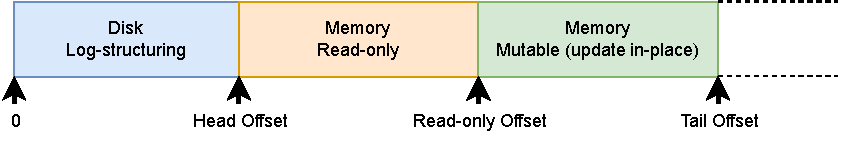
\includegraphics[width=0.9\textwidth]{logical-address-space.pdf}
    \caption{Logical Address Space used in HybridLog.}
    \label{fig:logical-address-space}
\end{figure}
\vspace{20px}

As records are written to the HybridLog, we first insert them to the tail of the ring buffer, we update the hash-index, and we move the tail offset further.
At every write, we also query the hash-index; if a key exists already in the mutable area, it is updated \textit{in-place}.
As we write new key-value pairs and the mutable area grows (because the tail offset moves towards higher logical addresses), we move the read-only offset too if needed, so that it stays behind the tail offset at a constant lag. This lag is configurable as an instantiation parameter of the HybridLog.

The records in the read-only area, as the name implies, are immutable. That is, when a write occurs on a key that is already present in that area, it is copied to the mutable area and updated there, which in the original work [\cite{faster}] is called a \textit{read-copy-update}. In our design we simplified a bit this procedure and we just do a new insert of the key-value pair with the new value in the mutable area.

Like with the read-only offset, we also maintain the head offset, which also has to stay at a constant lag behind the read-only offset, and this lag (or interval) is also configurable as an instantiation parameter.
When the gap in the logical addresses between the head offset and the read-only offset reaches the defined value of the interval, we flush all the read-only records to disk, i.e. the entire read-only area, and move the head offset to the last logical address that resides on disk, just before the read-only offset.

To retrieve a value, we first query the hash-index; if the key does not exist in the index, we just return the empty value (zero bytes). If the key exists and has a logical offset greater than the head offset, it lies in memory so we retrieve it from the ring buffer. If it resides on disk, we translate the offset appropriately and retrieve it from one of the files by doing a seek and a read operation.

The disk area is log-structured, in the same way that AppendLog is - they both use the same merging strategy for their files, and they both use the same value retrieval method to retrieve values from the files.

It is important to notice how the buffering policy acts like a cache for the writes.
The in-memory updates and the read-copy-update from the read-only area exploits the temporal locality of keys.
Therefore, this design choice should accelerate workloads with strong temporal locality. Also, the buffering stage does not require continuous flushing of the records by design, turning a succession of frequent small flushes into a large one. This behavior by itself yields faster writes. The downside of this (because no design choice comes without trade-offs) is that we have volatile records. If the system suddenly crushes, we inevitably lose the unflushed records.

To address the issue of potentially lost records, the authors of the original work [\cite{faster}] suggest using a write-ahead log as a workaround.
Similarly to the approach we took with the LSM-Tree, a write-ahead log can provide a reliable record of updates and help ensure data consistency in the event of system failures.
% authors also argue that the wal is not actually needed, checkpointing mechanism instead, but dont elaborate.

Regarding recovery after failures, the HybridLog does exactly what the AppendLog does to rebuild its hash-index; it scans all the runfiles in reverse order and points the index to the latest records.

\subsection{Implementation}

The implementation of the HybridLog essentially extends the implementation of the AppendLog by replacing the hash-index, adding the ring buffer, and also adding some logic to support the translation of the logical addresses.

\subsubsection{Hash-index}

The first step of our implementation is the hash-index. Because Python (the language of the implementation) does not allow low-level memory management, we had to simplify the design.
The simplified design can be seen in figure \ref{fig:hash-index}.
The index consists of a Python list that holds ``buckets''.
Each bucket is itself a list of length 8. The first 7 entries are integers, of which the upper bits hold the keys and the lower bits the values (which will be used to hold the logical addresses). The last entry holds the index of the next bucket, in case of overflow.
New buckets are allocated at the end of the list holding the buckets.

\vspace{20px}
\begin{figure}[h]
    \centering
    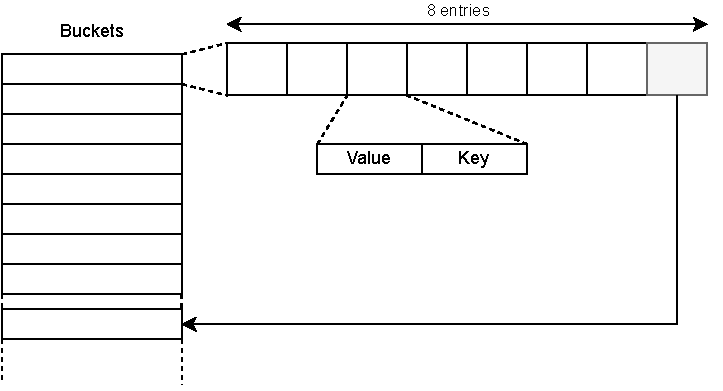
\includegraphics[width=0.9\textwidth]{hash-index.pdf}
    \caption{Hash-index of HybridLog.}
    \label{fig:hash-index}
\end{figure}
\vspace{20px}

To lookup a key in this hash-index, we hash it first using the MurmurHash3 hash function which is suitable for hash-based lookups, we calculate the modulo of the hash with the initial number of buckets, and then we follow the buckets, scanning the entries for the key, until we exhaust the buckets.

To insert or update a new key, we first perform a lookup. If we find the key in some bucket, we update its value. Otherwise, we scan for an empty space an insert the key-value pair. If there is no room, we allocate a new bucket and set the last bucket to point to it. When the inserted key-value pairs reach 75\% of the total capacity of the bucket, we resize it by allocating a new one with double the capacity ($2^{k+1}$ buckets if the previous one had $2^{k}$) and copy over the existing records. Deletion is implemented an update of the key's value to the empty value.

Another simplification that is necessary is the removal of the epoch-protection framework. Again, since we are working in Python and we do not have access to low-level threading capabilities, we did not implement the framework.

After implementing the simplified hash-index, we realized that it is actually quite slow, about three times slower than a Python dictionary. Upon reflection, the reduced performance appears to have been a predictable outcome, since it is implemented entirely in Python, while Python's dictionary is implemented in C and bypasses all the overhead that the high-level features of an interpreted language like Python add.

Thus, we continued the implementation using the Python dictionary as the backend for the hash-index. This choice, in addition to the dictionary being faster, is supported by two more reasons:
\begin{enumerate}
    \item It allows for fairer comparisons in the evaluations and comparisons in Chapter \ref{Chapter4-evaluation}, because the other engines also use the Python dictionary as a HashMap, especially AppendLog which uses the dictionary as its main index as well.
    \item We do not have any limitations about the key's length anymore.
\end{enumerate}

\subsubsection{Ring buffer}

After the hash-index implementation, our attention turned to the ring buffer.
This data structure is represented in Python as a list with two pointers, one for reading and one for writing, which wrap around the list in a circular fashion.
To achieve this, we calculate the respective buffer offsets using the modulo operation with the buffer's length.
This approach allows for efficient and continuous data processing within the buffer, without the need for costly buffer reallocations or data movement.

\subsubsection{Flushing and Merging}

Then, we implemented the logic for the flushing to disk, along with the log-structuring. Every time the lag between the head offset and the read-only offset reaches the corresponding predefined interval limit (given as a constructor argument), a flush occurs of the read-only area of the ring buffer. Each flush creates a new file. When the number of the files reaches a given threshold, a merge is triggered, which merges the files into one, placed in the next level in our log-structured setup, exactly like we do with the AppendLog.

The next checkpoint of the implementation is the logical address translation. The logical addresses need to be mapped to offsets of the ring buffer or offsets of files. For the ring buffer, the mapping is straightforward: we just use the modulo operator and the size of the buffer. For the disk, we used a Python dictionary which maps a logical offset to a specific offset of a specific file. This decision uses extra memory, but cannot be avoided. In \textsc{Faster}, the authors use an allocator which also uses extra memory behind the scenes. If we had only one logfile and entries with fixed length, we could have had a one-to-one address translation between the logical offsets and the file offsets by adding or subtracting a constant every time, but \textit{giving up on log-structuring and the freedom to use whatever length for our keys and values is not worth the trade-off}.

% concern: what happens with overflow of the 48bits?

\section{Snapshots}
\label{section-snapshots}

In the context of distributed systems, fault tolerance is central.
Replication is one of the most effective methods that systems employ to achieve fault tolerance. By storing copies of data across multiple nodes, replication can help ensure that the system remains available even if some of its nodes fail.

As we design state storage backends, it is important to provide the user with interfaces that allow for remote storage of the state and the ability to access different versions of that state. This includes the ability to roll back to previous versions of it if necessary.

In this section we will look into the method we implemented for creating snapshots efficiently from our log-structured key-value stores, as well storing them in remote storage, and restoring previous versions of it.

\subsection{Remotes}

First of all we define an abstraction we call \textit{Remote}.
The remote is an abstraction for remote storage.
The endpoints it exposes to the user are the following:

\begin{enumerate}
    \item \verb|put|: Uploads a file to the remote storage.
    \item \verb|get|: Fetches a file from the remote storage. By default it fetches the latest version but a previous version of it can be retrieved as well.
    \item \verb|gc|: Keeps only the files associated with the latest version and deletes the rest to free up storage space.
    \item \verb|restore|: Retrieves all the files associated with a given version.
    \item \verb|destroy|: Deletes the remote storage with all the files in it.
\end{enumerate}

The exact method signatures can be found in appendix \ref{Appendix-A-code}.

For the backend of the remotes we have two implementations: A directory in the local filesystem (to which a remote directory can be mounted) called \verb|PathRemote|, and a bucket in the S3 compatible object store \textit{minio} for the cloud called \verb|MinioRemote|.

To connect a remote storage to one of the key-value stores, the user creates an instance of a type of \verb|Remote| of choice and passes it as a constructor argument when instantiating the key-value store.

If a remote is given to a store, the store will prioritize it over local files for recovery. Instead of performing file discovery at the local data directory to rebuild the indices and the in-memory data-structures from the local pre-existing files, the store will query the remote for the latest version saved. If no version exists, the store starts anew, otherwise it fetches the files of the latest version and uses those to recover the state of that version.

\subsection{Incremental Snapshots}

The implementation of the incremental snapshotting functionality in a log-structured store is done with the use of \textit{delta maps}.

The general idea boils down to this: the store performs file discovery on its local directory and enumerates its local files in a set. It then queries the remote about the files it has stored and the remote sends those files in a different set. The store then calculates the difference between these two sets and then proceeds to ``push'' or ``pull'' the missing files, according to which operation is performed, snapshot or rollback respectively. This way, when the store takes a snapshot it will upload only new or changed files containing the recent writes, and if it is restoring a previous version from the remote, it will again only download the differences (the \textit{deltas}), avoiding repetition of work that is already done and hence making the snapshots and recoveries faster. Importantly, the store will flush any records reside in memory before taking a snapshot.

To implement this conceptually trivial procedure we need three things: a way to identify the changed files, a way to keep all the versions of all files in the remote without overwrites, and a way to associate each snapshot with a set of files and their versions. We can cover all three requirements with the following:

\begin{enumerate}
    \item We add a version counter to each instance of a key-value store called ``global version''. The value of this counter is appended to each runfile's filename and is incremented every time a merge takes place. To illustrate with an example, the file with name \verb|L0.0.run| after this addition will be \verb|L0.0.0.run|, and it will be different than the file with name \verb|L0.0.1.run| - the latter is created after a merge occurred in level 0. Deletions of files after merging are done as previously, without changes needed.
    \item Save all the filenames of a snapshot in a version-file in the remote and associate that file with the snapshot version by adding the snapshot version in the filename.
\end{enumerate}

When the store requests to perform a rollback to a specific version, it will read the version-file associated with the version to be restored and fetch all the relevant files. This can be done again with deltas trivially to be maximally efficient, like it is done in snapshots, but in our implementation we just delete the old files and fetch the files needed, for simplicity. Importantly, when recovering a previous snapshot, the global version of the store needs to be set to a value such that newer snapshots will not interfere with older ones. We choose this value to be the maximum global version detected in the remote files' names, which preserves this invariant and maintains the properties of snapshot and recovery we require in our design.

Incremental snapshotting is visualized in figure \ref{fig:incremental-snapshots}. In this example, the remote has saved a version comprised of the file \verb|L1.0.0.run|, which contains the merged changes from files \verb|L0.0.0.run|, \verb|L0.1.0.run| and \verb|L0.2.0.run|. When the store writes two new files, \verb|L0.0.1.run| and \verb|L0.1.1.run| and takes a snapshot at this point, it will only push these two to the remote, since the remote already has the file \verb|L1.0.0.run|.

\vspace{20px}
\begin{figure}[h]
    \centering
    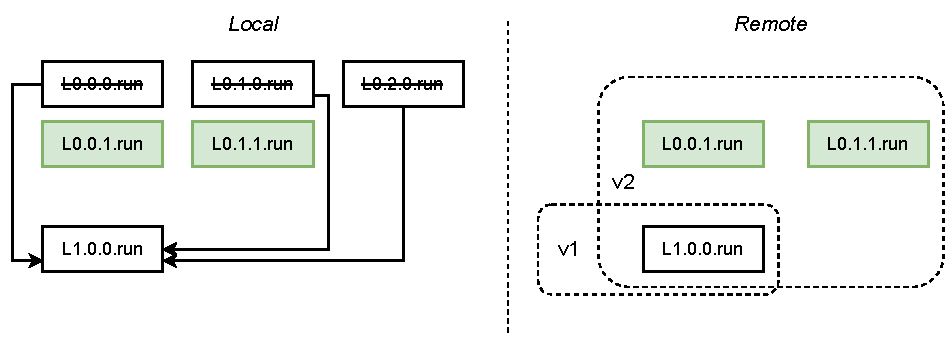
\includegraphics[width=0.9\textwidth]{incremental-snapshots.pdf}
    \caption{Incremental snapshotting example.}
    \label{fig:incremental-snapshots}
\end{figure}
\vspace{20px}

The global version addition we implemented also has a very convenient side effect: it allows us to execute merges in the background. Since this feature has not yet been implemented, we discuss it in the following section, \ref{section-extensions}.

\section{Possible extensions and optimizations}
\label{section-extensions}

In this section, we will explore a range of potential extensions and optimizations for the implemented key-value store engines. We will begin by focusing on LSM-Tree-specific additions and modifications, followed by an examination of optimizations that can be applied to all engine types.

\subsection{LSM-Tree}

The implemented LSM-Tree uses a write-ahead-log (WAL) to ensure that buffered records are never lost. However, this reduces the performance of the writes, as each write must be written to disk instead of solely being added to memtable.

The trade-off is worth it in the general use-case, but probably not for our use-case. This fault-tolerance property is at the level of local storage. In a distributed system, where snapshots are stored in different stores remotely, the WAL may be redundant. In a future version of the key-value store implementation it will be made optional.

At the core of the LSM-Tree, there are a number of optimizations that can be implemented to increase performance:

\begin{enumerate}
    \item The false-positive probability of the Bloom filters can be tweaked by dynamically allocating memory in order to optimally balance the costs between updates and lookups [\cite{lsm-monkey}].
    \item The merge frequency can be adapted to remove superfluous merges based on the workload and hardware [\cite{lsm-dostoevsky}]
    \item By setting increasing capacity ratios (which are functions of the number of runs at each level) between smaller levels, newer data can be merged more easily, leading to faster writes [\cite{lsm-wacky}].
    \item The segments defined by the fence pointers can be compressed using an online lossless compression algorithm like the LZW algorithm [\cite{lzw}] to increase disk-space efficiency.
    \item Bloom filters can be added per-level instead of per-file, or added alongside them, to potentially skip entire levels when looking up values in tiered LSM-Trees and substantially boost read performance.
\end{enumerate}

The aforementioned improvements naturally come with a resource trade-off, as their implementation necessitates increased memory usage, larger disk space requirements, or both.

\subsection{Improvements for all engines}

There are several key optimizations that can be universally applied to all three engines:

\begin{enumerate}
    \item The process of merging files can be trivially executed in the background, particularly leveraging the mechanism of versioned files we implemented for the incremental snapshotting functionality.

    \item It is imperative to enable concurrent reads while writing to the engines for enhanced performance.

    \item When it comes to writing to files, especially those that involve Bloom filters, the implementation of memory mapped I/O could yield significant benefits. This technique involves mapping files directly into the system's memory, enabling faster and more efficient data transfer between the application and the storage.

    \item To ensure data integrity and prevent any potential data corruption, we could augment each record with a small metadata field that includes a checksum. This can be done for example by appending one byte at the end of every record. This additional information allows for the verification of data integrity.

    \item In order to enhance ``analytics readiness'', i.e. the ability to perform aggregations on the data stored, there is an improvement that can be implemented. To perform analytics on the data in a scalable manner, the files need to be independently scannable. To scan each file independently, we should avoid querying any indices. To achieve that, an easy way is through incorporating a ``tombstone'' (see \ref{api}) within the metadata of each record. This tombstone serves as a marker, indicating the presence of invalid or irrelevant records, thereby allowing for the exclusion of such records without the need to query any indexing mechanism.

    \item Compression can be applied to the remotes for more efficient disk-space utilization.
\end{enumerate}
